%\documentclass{article}
\documentclass[12pt,a4paper,oneside]{book}
\usepackage[subpreambles=true]{standalone}
\usepackage{import}
\usepackage[T1]{fontenc}
\usepackage{times}
\usepackage[utf8]{inputenc}
\usepackage{amsmath}
%\usepackage{graphicx}
\usepackage{multicol}
\usepackage{longtable}
\usepackage[refpages]{gloss}
\usepackage{float}
\usepackage{anysize}
\usepackage{appendix}
\usepackage{lscape} 
\usepackage{pdflscape}
\usepackage{multirow}
\usepackage{listings}
\usepackage{color}
\usepackage{setspace}
\usepackage{enumerate} 
\usepackage{pdfpages}
\usepackage{lipsum}



\title{Proyecto Final de estudio }
\author{ANDER EGG Marcos, ARTERO Francisco, GAMBINO Ignacio}
\date{Octubre 2023}

\begin{document}

%----------------------------------------------------------------------------------------
%	CONFIGURACION
%----------------------------------------------------------------------------------------

\marginsize{3.0cm}{3.0cm}{4.0cm}{3.0cm}
\renewcommand*{\contentsname}{ÍNDICE}
\renewcommand*{\listtablename}{Índice de tablas}
\renewcommand*{\listfigurename}{Índice de figuras}
\renewcommand{\baselinestretch}{1.0}
\renewcommand{\appendixname}{Anexos}
\renewcommand{\appendixtocname}{Anexos}
\renewcommand{\appendixpagename}{Anexos}
\renewcommand{\thetable}{\arabic{chapter}.\arabic{table}}
\renewcommand*{\tablename}{Tabla}
\renewcommand*{\chaptername}{Capítulo}
\renewcommand*{\thechapter}{\Roman{chapter}}
\renewcommand{\thesection}{\arabic{chapter}.\arabic{section}}
\renewcommand{\figurename}{Figura}
\renewcommand{\thefigure}{\arabic{chapter}.\arabic{figure}}
\renewcommand{\theequation}{\arabic{chapter}.\arabic{equation}}



%----------------------------------------------------------------------------------------
%	PORTADA
%----------------------------------------------------------------------------------------

\begin{titlepage}
 
\begin{center}
 
 {\huge \bf UNIVERSIDAD NACIONAL DE CUYO}\\[1.2cm]
 
{\Large PROYECTO FINAL DE ESTUDIO}\\{\Large  -  Facultad de Ingeniería - Carrera Ingeniería Industrial -}\\[2.0cm]


\begin{center}

\includegraphics[width=0.35\textwidth]{images/escudo-uncuyo.png}
\end{center}

\vspace{1.7cm}
{{\bf Título: }: }Carbón activado a base de residuos organicos
\title{Carbon activado a base de residuo vegetal} % titulo de tu tesis para latex
{\bf \large . }\\[1.7cm] % titulo de tu tesis


{EJEMPLAR DE TESIS PRESENTADO PARA OPTAR EL TÍTULO DE INGENIERO INDUSTRIAL}\\[0.5cm]
 
{{\bf Autores}: }\\[0.5cm] % nombres del autor o autores

{\large ANDER EGG Marcos - ARTERO Francisco - GAMBINO Ignacio  - Julio
2023}\\[0.8cm] % fecha de sustentación
{Mendoza - Argentina}
\end{center}

\end{titlepage}

\newpage
\newpage
$\ $
\thispagestyle{empty} % para que no se muestre el número en la página

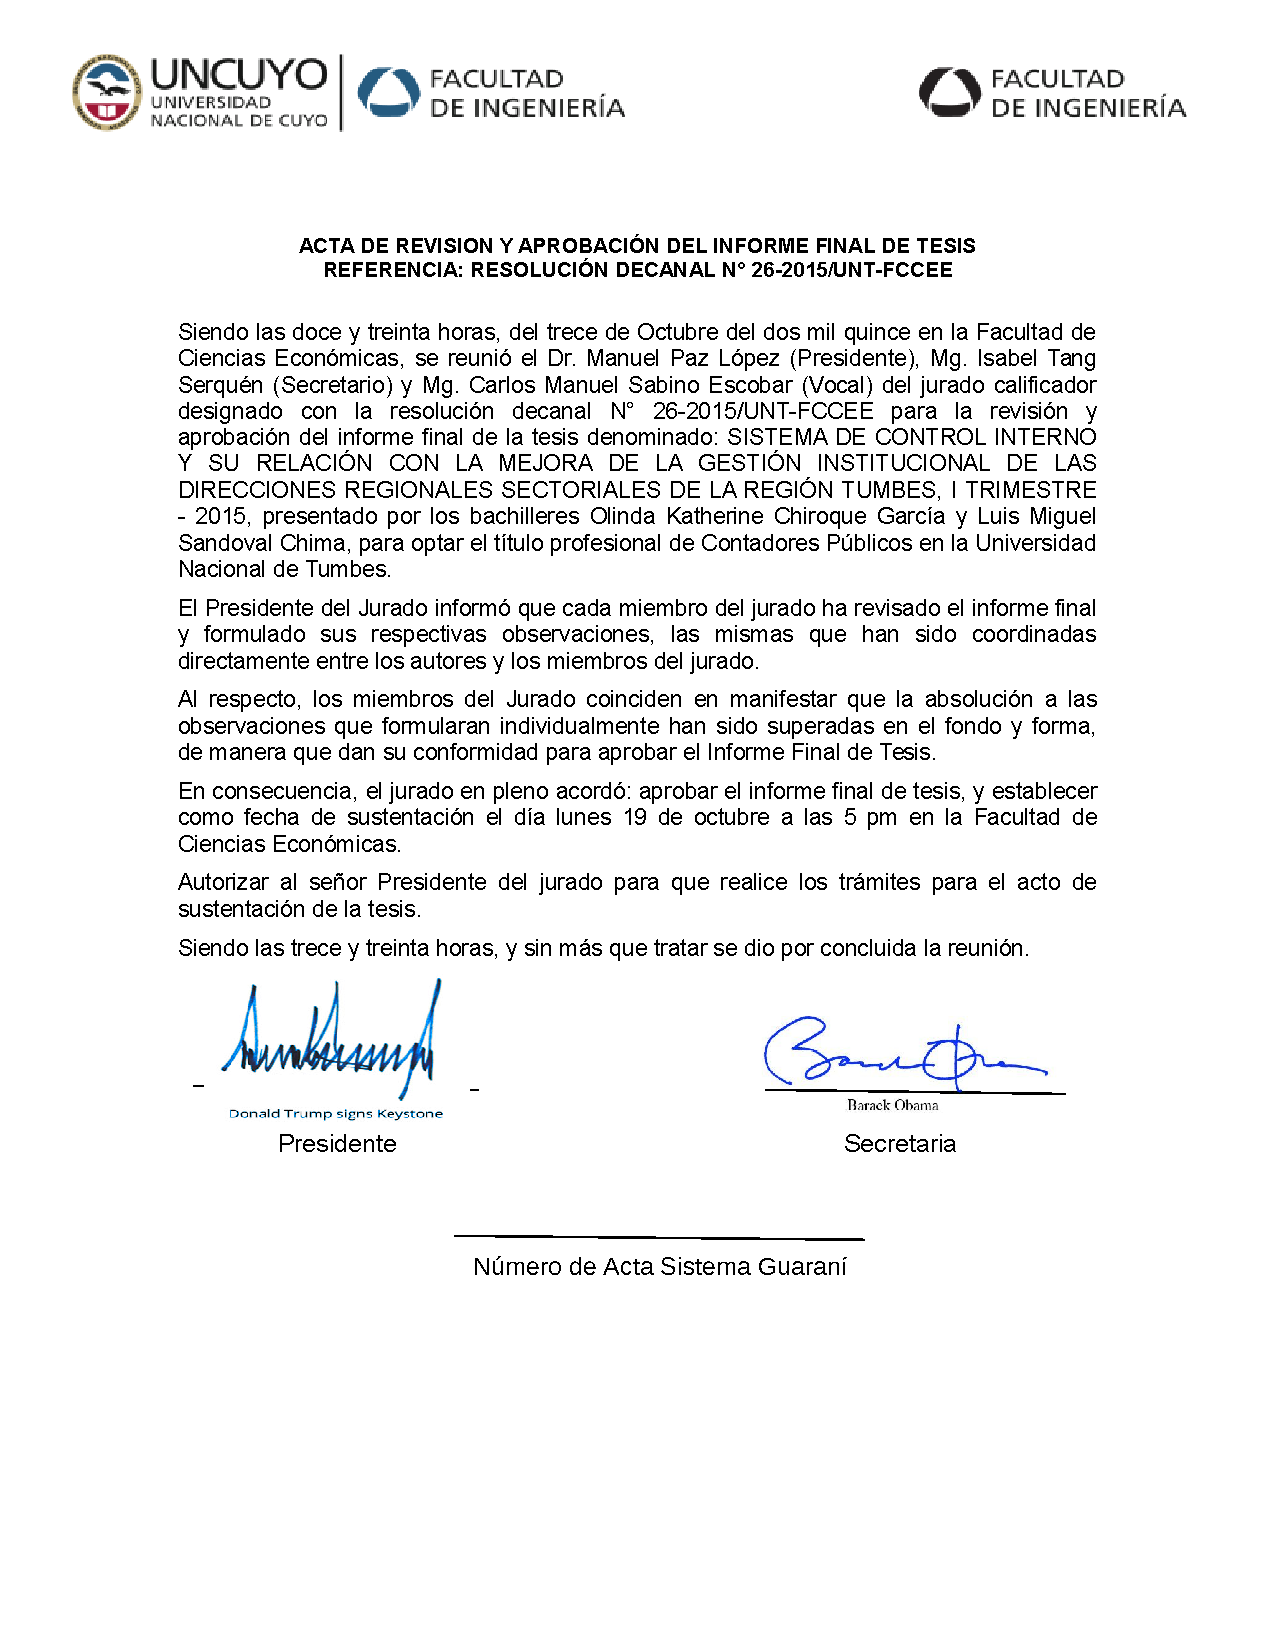
\includepdf{ACTAS/ACTA-TESIS}%se incluye un PDF con firmas o cualquier otro documento



%----------------------------------------------------------------------------------------
%	Dedicatoria
%----------------------------------------------------------------------------------------

\begin{titlepage}

\begin{flushright}
{\large \bf DEDICATORIA}
\\
\textit{}
\\
\textit{} % agregar tu dedicatoria
\end{flushright}
\end{titlepage}

%----------------------------------------------------------------------------------------
%	Agradecimientos
%----------------------------------------------------------------------------------------

\begin{titlepage}

\begin{flushright}
{\large \bf AGRADECIMIENTO}
\\
\textit{}
{} % agregar tu dedicatoria
\end{flushright}
\end{titlepage}


%----------------------------------------------------------------------------------------
%	TABLA DE CONTENIDOS
%---------------------------------------------------------------------------------------

\tableofcontents
\cleardoublepage
\listoftables
\listoffigures 
%\makegloss
\newpage

%----------------------------------------------------------------------------------------
%	Resumen
%----------------------------------------------------------------------------------------




%\maketitle

\chapter{Introducción}

\section{Contexto de la producción de carbón vegetal activado}

\section{Justificación de la elección de desechos de la industria vitivinícola}

\section{Objetivos del proyecto}

\chapter{Revisión de la Literatura}

\section{Carbón vegetal activado: concepto y aplicaciones}

\section{Desechos orgánicos en la industria vitivinícola}

\section{Procesos de producción de carbón vegetal activado}

\section{Estudios previos relacionados con la producción de carbón activado a partir de desechos vitivinícolas}

\chapter{Caracterización de los Desechos Vitivinícolas}

\section{Tipos de desechos generados en la industria vitivinícola}

\section{Composición química de los desechos}

\section{Disponibilidad y acceso a los desechos}

\section{Potencial de los desechos para la producción de carbón activado}

\chapter{Proceso de Producción de Carbón Vegetal Activado}

\section{Pretratamiento de los desechos}

\section{Proceso de carbonización}

\section{Activación del carbón}

\section{Caracterización del carbón activado producido}

\chapter{Evaluación de Propiedades del Carbón Activado}

\section{Área superficial específica}

\section{Porosidad}

\section{Actividad química}

\section{Aplicaciones Potenciales del Carbón Activado}

\section{Uso en la industria vitivinícola}

\section{Aplicaciones en otras industrias}

\section{Aspectos medioambientales}

\chapter{Evaluación Económica}

\section{Análisis de costos de producción}

\section{Proyección de ingresos}

\section{Análisis de viabilidad económica}


\chapter{Impacto Ambiental}

\section{Evaluación del ciclo de vida}

\section{Comparación con métodos de eliminación de desechos convencionales}


\chapter{Conclusiones y Recomendaciones}

\section{Resumen de los hallazgos clave}

\section{Implicaciones y perspectivas futuras}

\section{Recomendaciones para la implementación práctica}

\chapter{Bibliografía}

\section{Referencias bibliográficas y fuentes consultadas}

\chapter{Anexos}

\section{Datos adicionales, gráficos, tablas, fotografías, etc.}



%\chapter{Financiamiento y Organización}
%\import{sections/}{section10}

%\chapter{Evaluación}
%\import{sections/}{section11}


\end{document}
